\documentclass{beamer}

%
% Common preamble for all three parts.
%

\usepackage[brazil,english]{babel}
\usepackage[utf8]{inputenc}
\usepackage{amsmath}
\usepackage{color}
\usepackage{minted}
\usepackage{hyperref}
\usepackage{multicol}
\usepackage{tabularx}
\usepackage{tikz}

% only inline todonotes work
\usepackage{xkeyval}
\usepackage[textsize=small]{todonotes}
\presetkeys{todonotes}{inline}{}

\usetikzlibrary{shapes,arrows,positioning,shadows}

% no nav buttons
\usenavigationsymbolstemplate{}

\newcommand{\bftt}[1]{\textbf{\texttt{#1}}}
\newcommand{\comment}[1]{{\color[HTML]{008080}\textit{\textbf{\texttt{#1}}}}}
\newcommand{\cmd}[1]{{\color[HTML]{008000}\bftt{#1}}}
\newcommand{\bs}{\char`\\}
\newcommand{\cmdbs}[1]{\cmd{\bs#1}}
\newcommand{\lcb}{\char '173}
\newcommand{\rcb}{\char '175}
\newcommand{\cmdbegin}[1]{\cmdbs{begin\lcb}\bftt{#1}\cmd{\rcb}}
\newcommand{\cmdend}[1]{\cmdbs{end\lcb}\bftt{#1}\cmd{\rcb}}

\newcommand{\wllogo}{\textbf{write\textrm{\LaTeX}}}

% this is where the example source files are loaded from
% do not include a trailing slash
%\newcommand{\fileuri}{https://raw.github.com/jdleesmiller/latex-course/master/en}
\newcommand{\fileuri}{https://raw.githubusercontent.com/jmetzz/latex-course/master/pt-br}

\newcommand{\wlserver}{https://www.writelatex.com}
\newcommand{\wlnewdoc}[1]{\wlserver/docs?snip\_uri=\fileuri/#1\&splash=none}

\def\tikzname{Ti\emph{k}Z}

% from http://tex.stackexchange.com/questions/5226/keyboard-font-for-latex
\newcommand*\keystroke[1]{%
  \tikz[baseline=(key.base)]
    \node[%
      draw,
      fill=white,
      drop shadow={shadow xshift=0.25ex,shadow yshift=-0.25ex,fill=black,opacity=0.75},
      rectangle,
      rounded corners=2pt,
      inner sep=1pt,
      line width=0.5pt,
      font=\scriptsize\sffamily
    ](key) {#1\strut}
  ;
}
\newcommand{\keystrokebftt}[1]{\keystroke{\bftt{#1}}}

% stolen from minted.dtx
\newenvironment{exampletwoup}
  {\VerbatimEnvironment
   \begin{VerbatimOut}{example.out}}
  {\end{VerbatimOut}
   \setlength{\parindent}{0pt}
   \fbox{\begin{tabular}{l|l}
   \begin{minipage}{0.55\linewidth}
     \inputminted[fontsize=\small,resetmargins]{latex}{example.out}
   \end{minipage} &
   \begin{minipage}{0.35\linewidth}
     \input{example.out}
   \end{minipage}
   \end{tabular}}}

\newenvironment{exampletwouptiny}
  {\VerbatimEnvironment
   \begin{VerbatimOut}{example.out}}
  {\end{VerbatimOut}
   \setlength{\parindent}{0pt}
   \fbox{\begin{tabular}{l|l}
   \begin{minipage}{0.55\linewidth}
     \inputminted[fontsize=\scriptsize,resetmargins]{latex}{example.out}
   \end{minipage} &
   \begin{minipage}{0.35\linewidth}
     \setlength{\parskip}{6pt plus 1pt minus 1pt}%
     \raggedright\scriptsize\input{example.out}
   \end{minipage}
   \end{tabular}}}

\newenvironment{exampletwouptinynoframe}
  {\VerbatimEnvironment
   \begin{VerbatimOut}{example.out}}
  {\end{VerbatimOut}
   \setlength{\parindent}{0pt}
   \begin{tabular}{l|l}
   \begin{minipage}{0.55\linewidth}
     \inputminted[fontsize=\scriptsize,resetmargins]{latex}{example.out}
   \end{minipage} &
   \begin{minipage}{0.35\linewidth}
     \setlength{\parskip}{6pt plus 1pt minus 1pt}%
     \raggedright\scriptsize\input{example.out}
   \end{minipage}
   \end{tabular}}

\title{Uma Introdução Interativa ao \LaTeX}
\author{Dr John D. Lees-Miller}


\titlegraphic{%

\includegraphics[page=4]{wllogo-series}\\[1em]

\includegraphics[height=24pt]{UoB-logo}
\qquad

\includegraphics[height=24pt]{setsquared_supported}
}



\subtitle{Parte 2: Documentos Estruturados \& Mais}

\begin{document}

%%%%%%%%%%%%%%%%%%%%%%%%%%%%%%%%%%%%%%%%%%%%%%%%%%%%%%%%%%%%%%%%%%%%%%%%%%%%%%%
%%%%%%%%%%%%%%%%%%%%%%%%%%%%%%%%%%%%%%%%%%%%%%%%%%%%%%%%%%%%%%%%%%%%%%%%%%%%%%%
%%%%%%%%%%%%%%%%%%%%%%%%%%%%%%%%%%%%%%%%%%%%%%%%%%%%%%%%%%%%%%%%%%%%%%%%%%%%%%%
\begin{frame}
\titlepage
\end{frame}

\begin{frame}

\begin{center}
Tradu\c{c}\~ ao por: Jean Metz

\textcolor{gray}{\href{http://www.jean.metzz.org/}{My homepage}}

\vskip 10ex



\includegraphics[height=24pt]{UTFPR-logo}
\end{center}

\end{frame}


%%%%%%%%%%%%%%%%%%%%%%%%%%%%%%%%%%%%%%%%%%%%%%%%%%%%%%%%%%%%%%%%%%%%%%%%%%%%%%%
%%%%%%%%%%%%%%%%%%%%%%%%%%%%%%%%%%%%%%%%%%%%%%%%%%%%%%%%%%%%%%%%%%%%%%%%%%%%%%%
%%%%%%%%%%%%%%%%%%%%%%%%%%%%%%%%%%%%%%%%%%%%%%%%%%%%%%%%%%%%%%%%%%%%%%%%%%%%%%%
\section{Documentos Estruturados}

%%%%%%%%%%%%%%%%%%%%%%%%%%%%%%%%%%%%%%%%%%%%%%%%%%%%%%%%%%%%%%%%%%%%%%%%%%%%%%%
%%%%%%%%%%%%%%%%%%%%%%%%%%%%%%%%%%%%%%%%%%%%%%%%%%%%%%%%%%%%%%%%%%%%%%%%%%%%%%%
%%%%%%%%%%%%%%%%%%%%%%%%%%%%%%%%%%%%%%%%%%%%%%%%%%%%%%%%%%%%%%%%%%%%%%%%%%%%%%%
\begin{frame}{Conteúdo}
\begin{multicols}{2}
\tableofcontents[currentsection]
\end{multicols}
\end{frame}

%%%%%%%%%%%%%%%%%%%%%%%%%%%%%%%%%%%%%%%%%%%%%%%%%%%%%%%%%%%%%%%%%%%%%%%%%%%%%%%
%%%%%%%%%%%%%%%%%%%%%%%%%%%%%%%%%%%%%%%%%%%%%%%%%%%%%%%%%%%%%%%%%%%%%%%%%%%%%%%
%%%%%%%%%%%%%%%%%%%%%%%%%%%%%%%%%%%%%%%%%%%%%%%%%%%%%%%%%%%%%%%%%%%%%%%%%%%%%%%
\begin{frame}{\insertsection}
	\begin{itemize}
		\item Na Parte 1, aprendemos sobre comandos e ambientes para composição de texto e fórmulas matemáticas.
		\item Agora, aprenderemos sobre comandos e ambientes para estruturar documentos.
		\item Você pode testar os novos comandos no write\LaTeX{}:
	\end{itemize}
	\vskip 2em
	\begin{center}
		\fbox{\href{\wlnewdoc{basics.tex}}{%
		Clique aqui para abrir o documento de exemplo no \wllogo{}}}
		\\[1ex]\scriptsize{}Ou vá para essa URL: \url{http://bit.ly/WU0bMU}\\
		Para melhor resultado, use \href{http://www.google.com/chrome}{Google Chrome} ou uma versão recente do \href{http://www.mozilla.org/en-US/firefox/new/}{FireFox}.
	\end{center}
	\vskip 2ex
	\begin{itemize}
		\item Vamos começar!
	\end{itemize}
\end{frame}

%%%%%%%%%%%%%%%%%%%%%%%%%%%%%%%%%%%%%%%%%%%%%%%%%%%%%%%%%%%%%%%%%%%%%%%%%%%%%%%
%%%%%%%%%%%%%%%%%%%%%%%%%%%%%%%%%%%%%%%%%%%%%%%%%%%%%%%%%%%%%%%%%%%%%%%%%%%%%%%
%%%%%%%%%%%%%%%%%%%%%%%%%%%%%%%%%%%%%%%%%%%%%%%%%%%%%%%%%%%%%%%%%%%%%%%%%%%%%%%
\subsection{Título e Resumo}
\begin{frame}[fragile]{\insertsubsection}
	\begin{itemize}{\small
		\item Diga ao \LaTeX{} o \cmdbs{title} e nome do \cmdbs{author} no preâmbulo.
		\item Então use \cmdbs{maketitle} no documento para criar de fato o título.
		\item Use o ambiente \bftt{abstract} para criar o resumo do documento.
	}
	\end{itemize}
	\begin{minipage}{0.45\linewidth}
		\inputminted[fontsize=\tiny,frame=single,resetmargins]{latex}%
		  {structure-title.tex}
	\end{minipage}
	\begin{minipage}{0.45\linewidth}
	\fbox{
		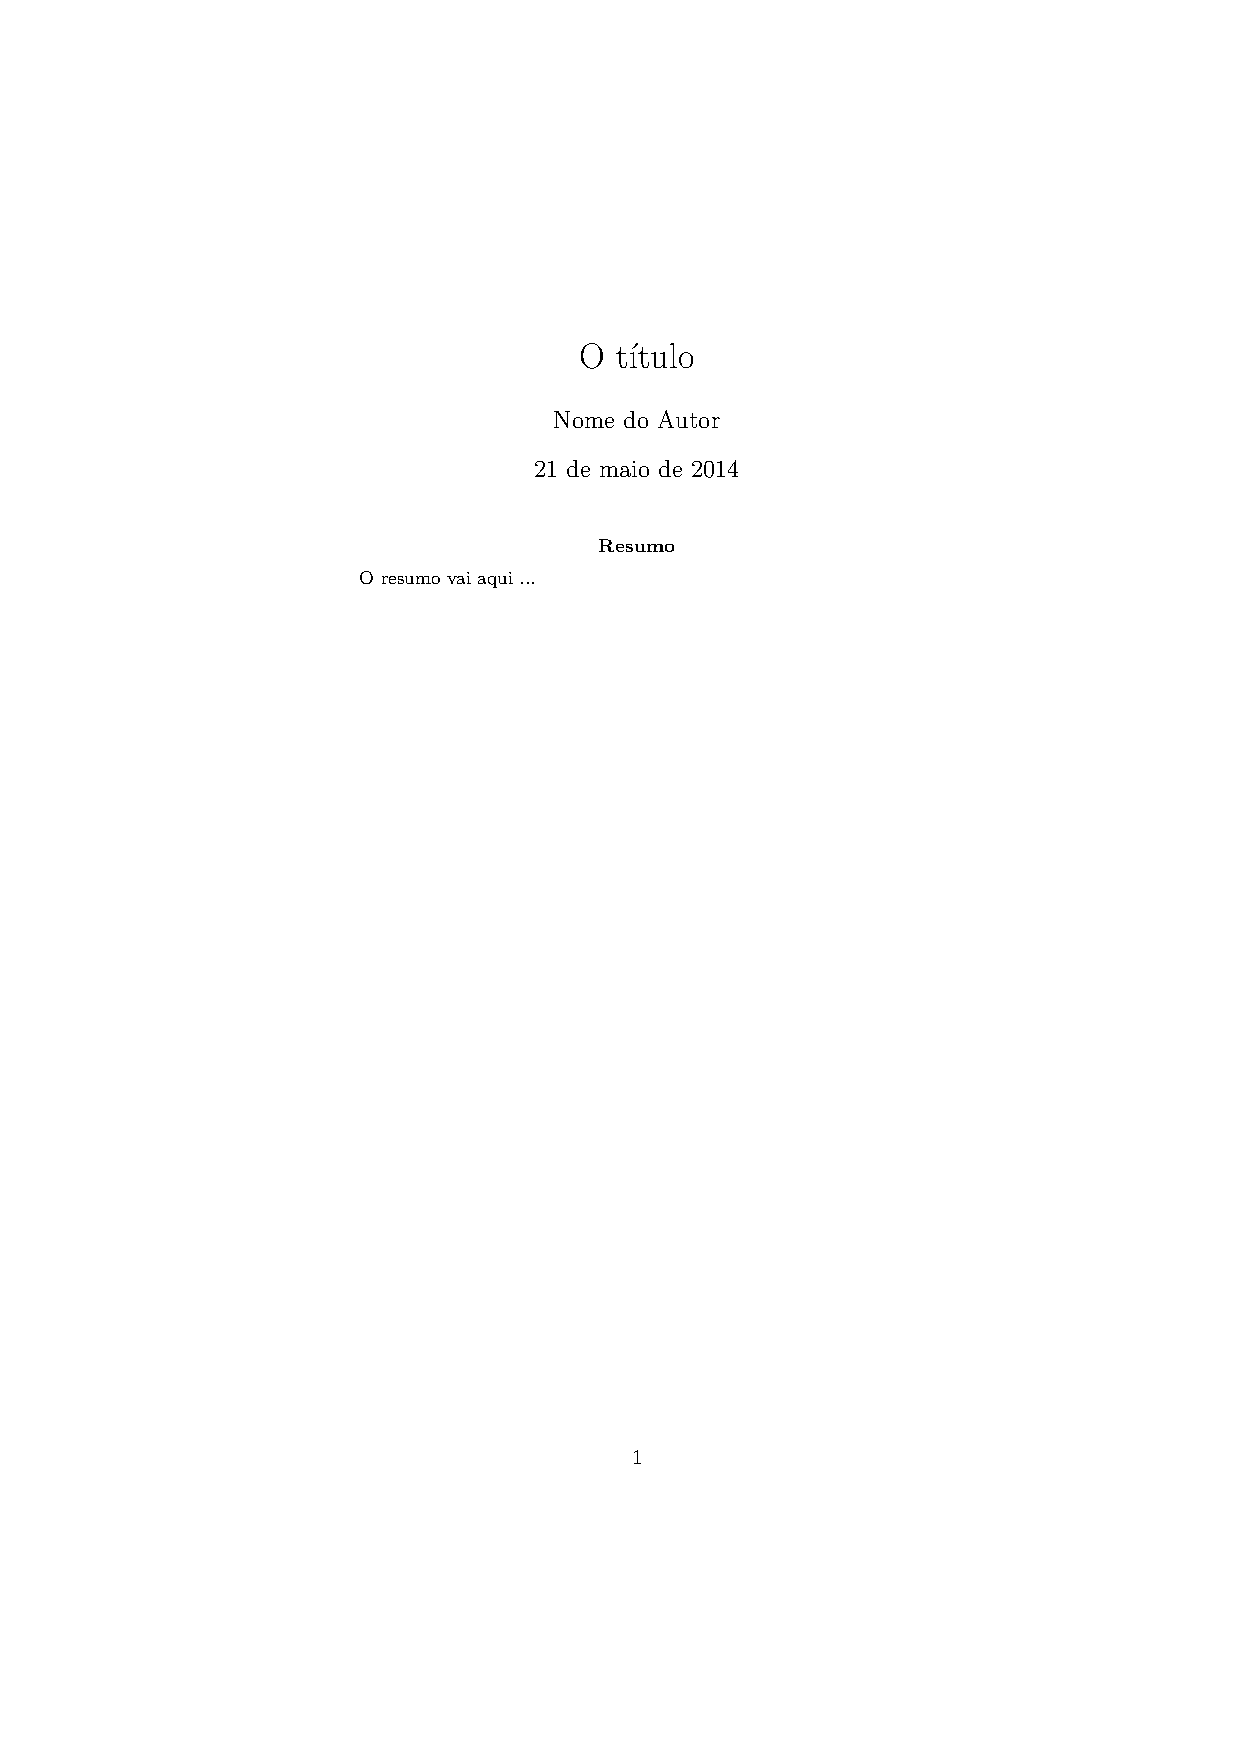
\includegraphics[width=\textwidth,clip,trim=2.2in 7in 2.2in 1.4in]{structure-title.pdf}}
	\end{minipage}
\end{frame}

%%%%%%%%%%%%%%%%%%%%%%%%%%%%%%%%%%%%%%%%%%%%%%%%%%%%%%%%%%%%%%%%%%%%%%%%%%%%%%%
%%%%%%%%%%%%%%%%%%%%%%%%%%%%%%%%%%%%%%%%%%%%%%%%%%%%%%%%%%%%%%%%%%%%%%%%%%%%%%%
%%%%%%%%%%%%%%%%%%%%%%%%%%%%%%%%%%%%%%%%%%%%%%%%%%%%%%%%%%%%%%%%%%%%%%%%%%%%%%%
\subsection{Seções}
\begin{frame}{\insertsubsection}
	\begin{itemize}{\small
		\item Use apenas \cmdbs{section} e \cmdbs{subsection}.
		\item Consegue adivinhar o que \cmdbs{section*} e \cmdbs{subsection*} fazem?
	}\end{itemize}
	\begin{minipage}{0.55\linewidth}
		\inputminted[fontsize=\tiny,frame=single,resetmargins]{latex}%
		  {structure-sections.tex}
	\end{minipage}
	\begin{minipage}{0.35\linewidth}
	\fbox{
		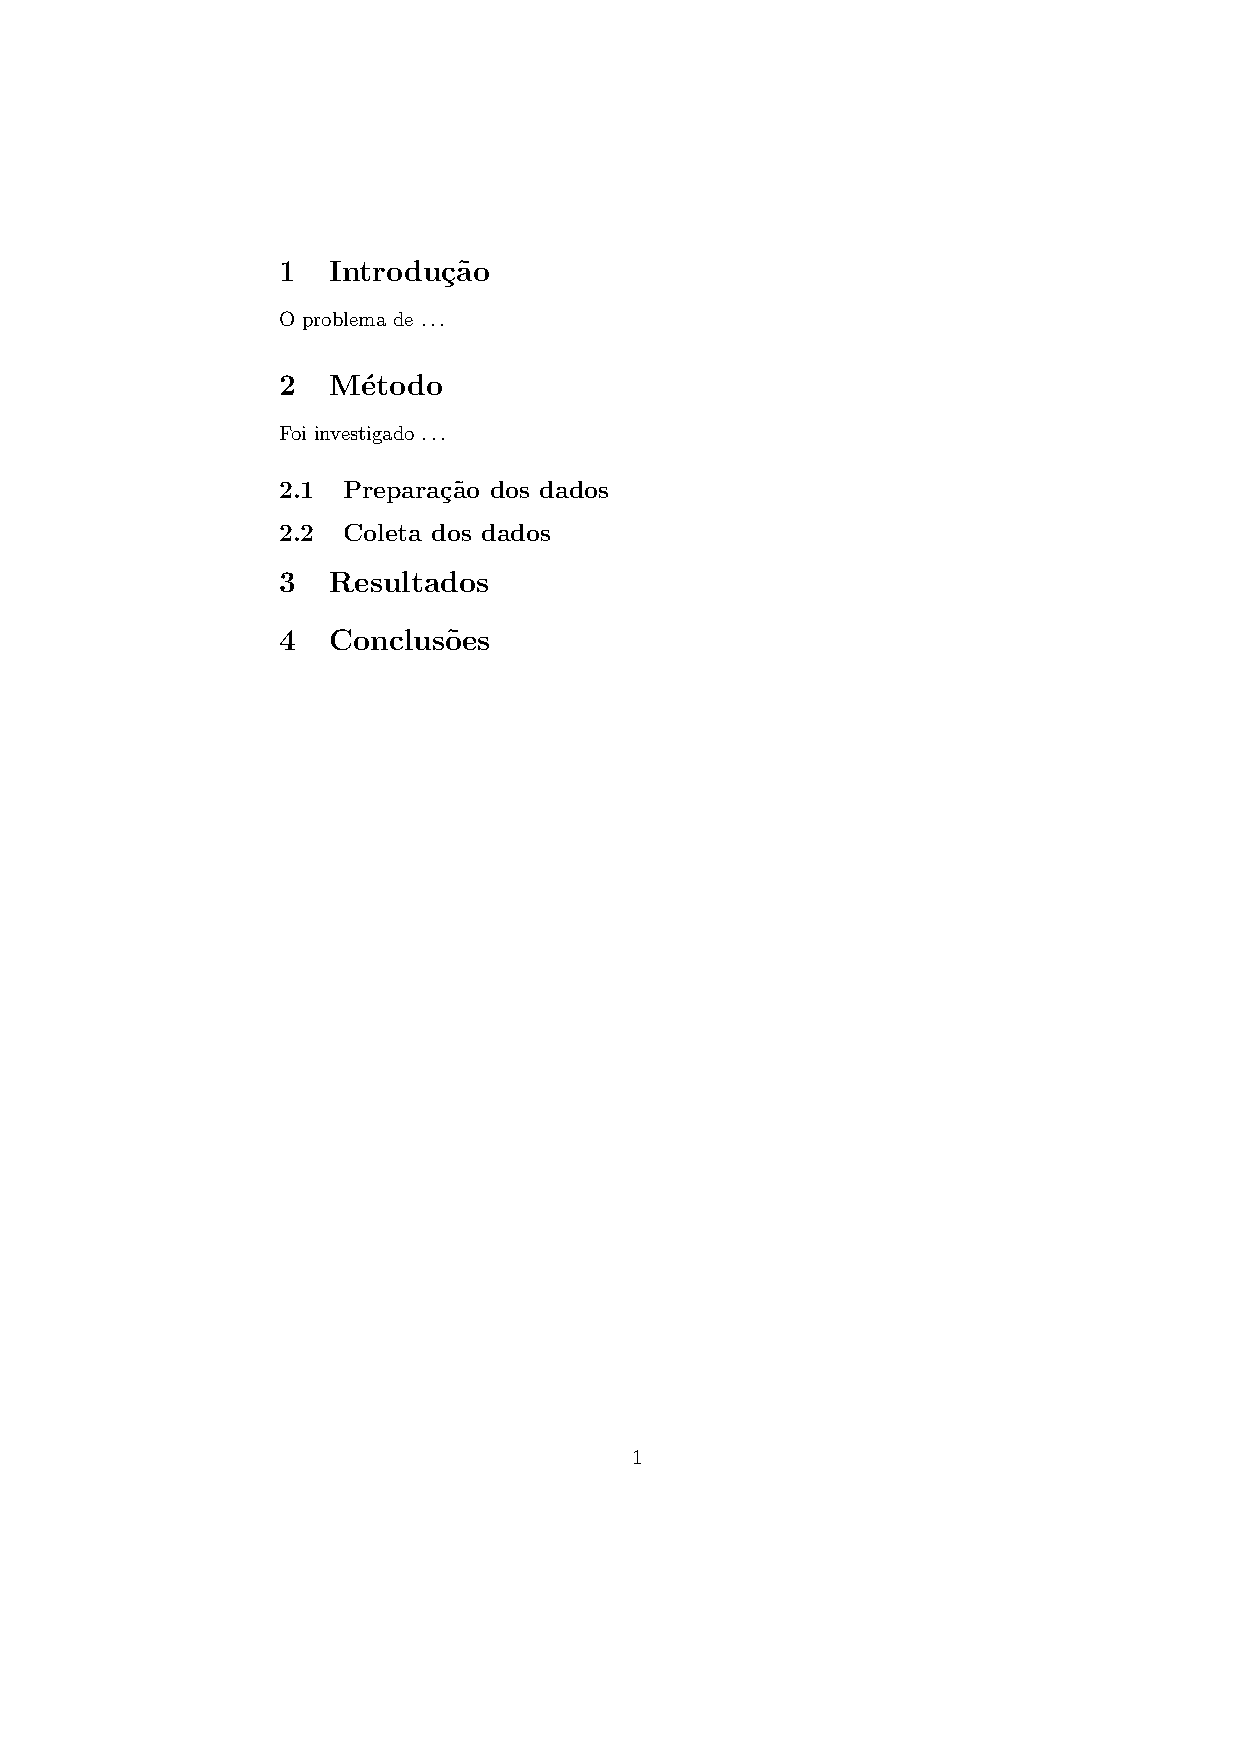
\includegraphics[width=\textwidth,clip,trim=2.2in 6.2in 2.2in 1in]{structure-sections.pdf}}
	\end{minipage}
\end{frame}

%%%%%%%%%%%%%%%%%%%%%%%%%%%%%%%%%%%%%%%%%%%%%%%%%%%%%%%%%%%%%%%%%%%%%%%%%%%%%%%
%%%%%%%%%%%%%%%%%%%%%%%%%%%%%%%%%%%%%%%%%%%%%%%%%%%%%%%%%%%%%%%%%%%%%%%%%%%%%%%
%%%%%%%%%%%%%%%%%%%%%%%%%%%%%%%%%%%%%%%%%%%%%%%%%%%%%%%%%%%%%%%%%%%%%%%%%%%%%%%
\subsection{Rótulos e referências cruzadas}
\begin{frame}[fragile]{\insertsubsection}
	\begin{itemize}{\small
		\item Use \cmdbs{label} e \cmdbs{ref} para numeração automática.
		\item O pacote \bftt{amsmath} provê \cmdbs{eqref} para referenciar equações.
	}\end{itemize}
	\begin{minipage}{0.55\linewidth}
		\inputminted[fontsize=\tiny,frame=single,resetmargins]{latex}%
		  {structure-crossref.tex}
	\end{minipage}
	\begin{minipage}{0.35\linewidth}
	\fbox{
		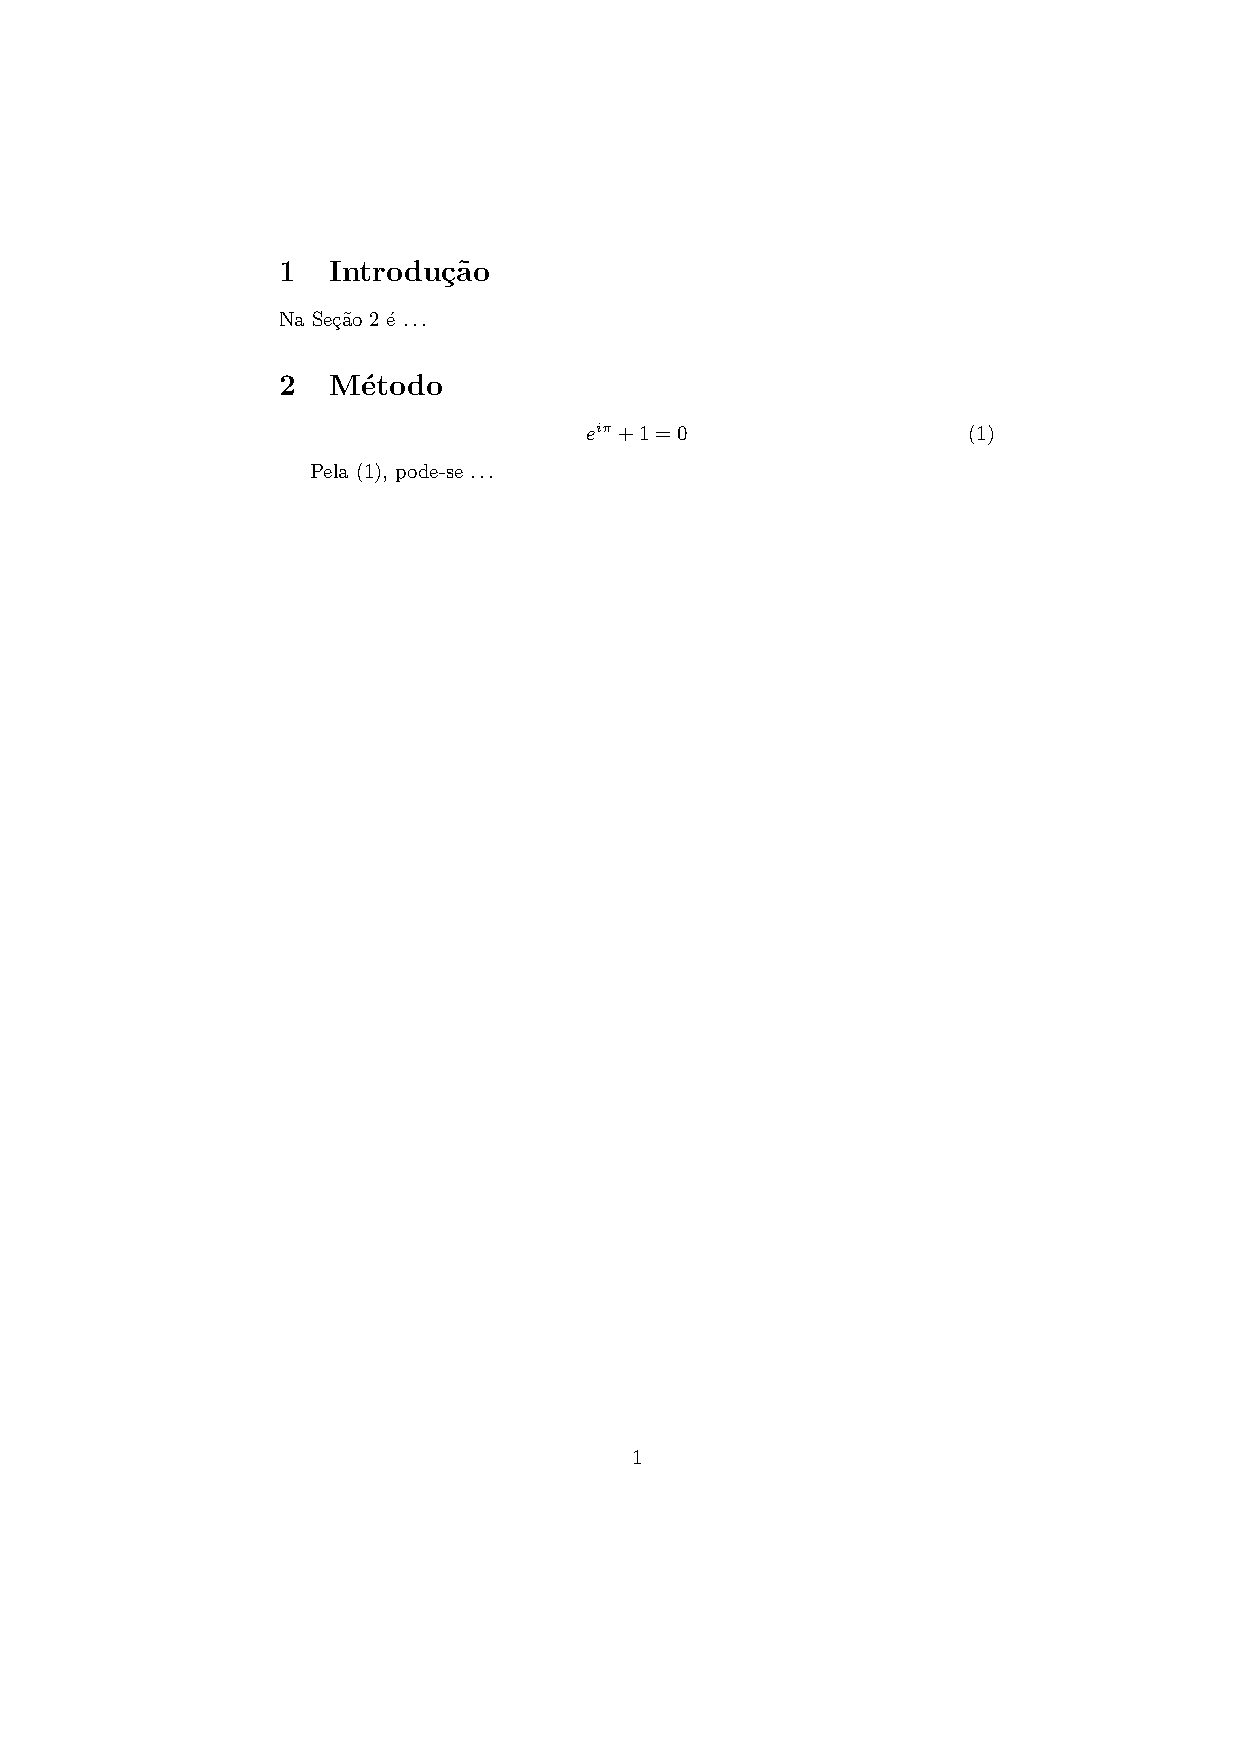
\includegraphics[width=\textwidth,clip,trim=1.8in 4.8in 1.6in 0in]{structure-crossref.pdf}}
	\end{minipage}
\end{frame}

%%%%%%%%%%%%%%%%%%%%%%%%%%%%%%%%%%%%%%%%%%%%%%%%%%%%%%%%%%%%%%%%%%%%%%%%%%%%%%%
%%%%%%%%%%%%%%%%%%%%%%%%%%%%%%%%%%%%%%%%%%%%%%%%%%%%%%%%%%%%%%%%%%%%%%%%%%%%%%%
%%%%%%%%%%%%%%%%%%%%%%%%%%%%%%%%%%%%%%%%%%%%%%%%%%%%%%%%%%%%%%%%%%%%%%%%%%%%%%%
\subsection{Exercício}
\begin{frame}[fragile]{Documentos Estruturados --- Exercício}

	\begin{block}{Digite esse artigo em \LaTeX:
	\footnote{Fonte \url{http://pdos.csail.mit.edu/scigen/}, um gerador de artigos aleatório.}}
	\begin{center}
	\fbox{\href{\fileuri/structure-exercise-solution.pdf}{%
	Clique aqui para abrir o artigo}}
	\end{center}
	Faça com que o seu artigo fique igual a esse. Use \cmdbs{ref} e \cmdbs{eqref} para evitar escrever explicitamente no texto os números de seções e equações.
	\end{block}
	\vskip 2ex
	\begin{center}
	\fbox{\href{\wlnewdoc{structure-exercise.tex}}{%
	Clique aqui para abrir este exercício no \wllogo{}}}
	\end{center}
	
	\begin{itemize}
	\item Uma vez que você tenha tentado,
	\fbox{\href{\wlnewdoc{structure-exercise-solution.tex}}{%
	clique aqui para ver a minha solução}}.
	\end{itemize}
\end{frame}

%%%%%%%%%%%%%%%%%%%%%%%%%%%%%%%%%%%%%%%%%%%%%%%%%%%%%%%%%%%%%%%%%%%%%%%%%%%%%%%
%%%%%%%%%%%%%%%%%%%%%%%%%%%%%%%%%%%%%%%%%%%%%%%%%%%%%%%%%%%%%%%%%%%%%%%%%%%%%%%
%%%%%%%%%%%%%%%%%%%%%%%%%%%%%%%%%%%%%%%%%%%%%%%%%%%%%%%%%%%%%%%%%%%%%%%%%%%%%%%
\section{Figures and Tables}

%%%%%%%%%%%%%%%%%%%%%%%%%%%%%%%%%%%%%%%%%%%%%%%%%%%%%%%%%%%%%%%%%%%%%%%%%%%%%%%
%%%%%%%%%%%%%%%%%%%%%%%%%%%%%%%%%%%%%%%%%%%%%%%%%%%%%%%%%%%%%%%%%%%%%%%%%%%%%%%
%%%%%%%%%%%%%%%%%%%%%%%%%%%%%%%%%%%%%%%%%%%%%%%%%%%%%%%%%%%%%%%%%%%%%%%%%%%%%%%
\begin{frame}{Conteúdo}
\begin{multicols}{2}
\tableofcontents[currentsection]
\end{multicols}
\end{frame}

%%%%%%%%%%%%%%%%%%%%%%%%%%%%%%%%%%%%%%%%%%%%%%%%%%%%%%%%%%%%%%%%%%%%%%%%%%%%%%%
%%%%%%%%%%%%%%%%%%%%%%%%%%%%%%%%%%%%%%%%%%%%%%%%%%%%%%%%%%%%%%%%%%%%%%%%%%%%%%%
%%%%%%%%%%%%%%%%%%%%%%%%%%%%%%%%%%%%%%%%%%%%%%%%%%%%%%%%%%%%%%%%%%%%%%%%%%%%%%%
\subsection{Gráficos}

\begin{frame}[fragile]{\insertsubsection}
	\begin{itemize}
		\item Requer o uso do pacote \bftt{graphicx}, no qual esté definido o 
		comando \cmdbs{includegraphics}.
		\item Os formatos de gráficos suportados incluem JPEG, PNG and PDF (usualmente). 
	\end{itemize}
	\begin{exampletwouptiny}
		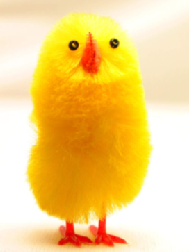
\includegraphics[width=0.5\textwidth]
		{big_chick}
		
		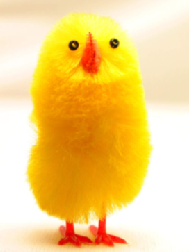
\includegraphics[width=0.3\textwidth,
						angle=270]{big_chick}
	\end{exampletwouptiny}
	
	\tiny{Imagem obtida em \url{http://www.andy-roberts.net/writing/latex/importing_images}}
\end{frame}

%%%%%%%%%%%%%%%%%%%%%%%%%%%%%%%%%%%%%%%%%%%%%%%%%%%%%%%%%%%%%%%%%%%%%%%%%%%%%%%
%%%%%%%%%%%%%%%%%%%%%%%%%%%%%%%%%%%%%%%%%%%%%%%%%%%%%%%%%%%%%%%%%%%%%%%%%%%%%%%
%%%%%%%%%%%%%%%%%%%%%%%%%%%%%%%%%%%%%%%%%%%%%%%%%%%%%%%%%%%%%%%%%%%%%%%%%%%%%%%
\begin{frame}[fragile]{Argumentos opcionais}
	\begin{itemize}
		\item Usamos colchetes \keystrokebftt{[} \keystrokebftt{]} para os argumentos opcionais, em vez de chaves \keystrokebftt{\{} \keystrokebftt{\}}.
		\item \cmdbs{includgraphics} aceita argumentos opcioanis que nos permite transformar a imagem quando são inclusos. Por exemplo, \bftt{width=0.3\cmdbs{textwidth}} faz com que a imagem fique com o tamanho de até 30\% da largura do texto (\cmdbs{textwidth}).
		\item \cmdbs{documentclass} aceita argumento opcionais, também. Exemplo: 
		\mint{latex}|\documentclass[12pt,twocolumn]{article}|
		\vskip 3ex
		altera a o tamanho da fonte para 12 pontos e distribui o texto em duas colunas.
		
		\item Onde encontrar mais informações sobre isso? Nos slides no final dessa apresentação há \textit{links} para páginas tratando sobre esse tema.
	\end{itemize}
\end{frame}

%%%%%%%%%%%%%%%%%%%%%%%%%%%%%%%%%%%%%%%%%%%%%%%%%%%%%%%%%%%%%%%%%%%%%%%%%%%%%%%
%%%%%%%%%%%%%%%%%%%%%%%%%%%%%%%%%%%%%%%%%%%%%%%%%%%%%%%%%%%%%%%%%%%%%%%%%%%%%%%
%%%%%%%%%%%%%%%%%%%%%%%%%%%%%%%%%%%%%%%%%%%%%%%%%%%%%%%%%%%%%%%%%%%%%%%%%%%%%%%
\subsection[fragile]{Ambientes flutuantes}
\begin{frame}{\insertsubsection}
	\begin{itemize}
		\item Permitem ao \LaTeX{} decidir onde a figura será posicionada (pode ``flutuar'').
		\item Você também pode atribuir uma legenda à figura, a qual pode ser referenciada com \cmdbs{ref}.
	\end{itemize}
	
	\begin{minipage}{0.55\linewidth}
		\inputminted[fontsize=\scriptsize,frame=single,resetmargins]{latex}%
	  {media-graphics.tex}
	\end{minipage}	
	\begin{minipage}{0.35\linewidth}
		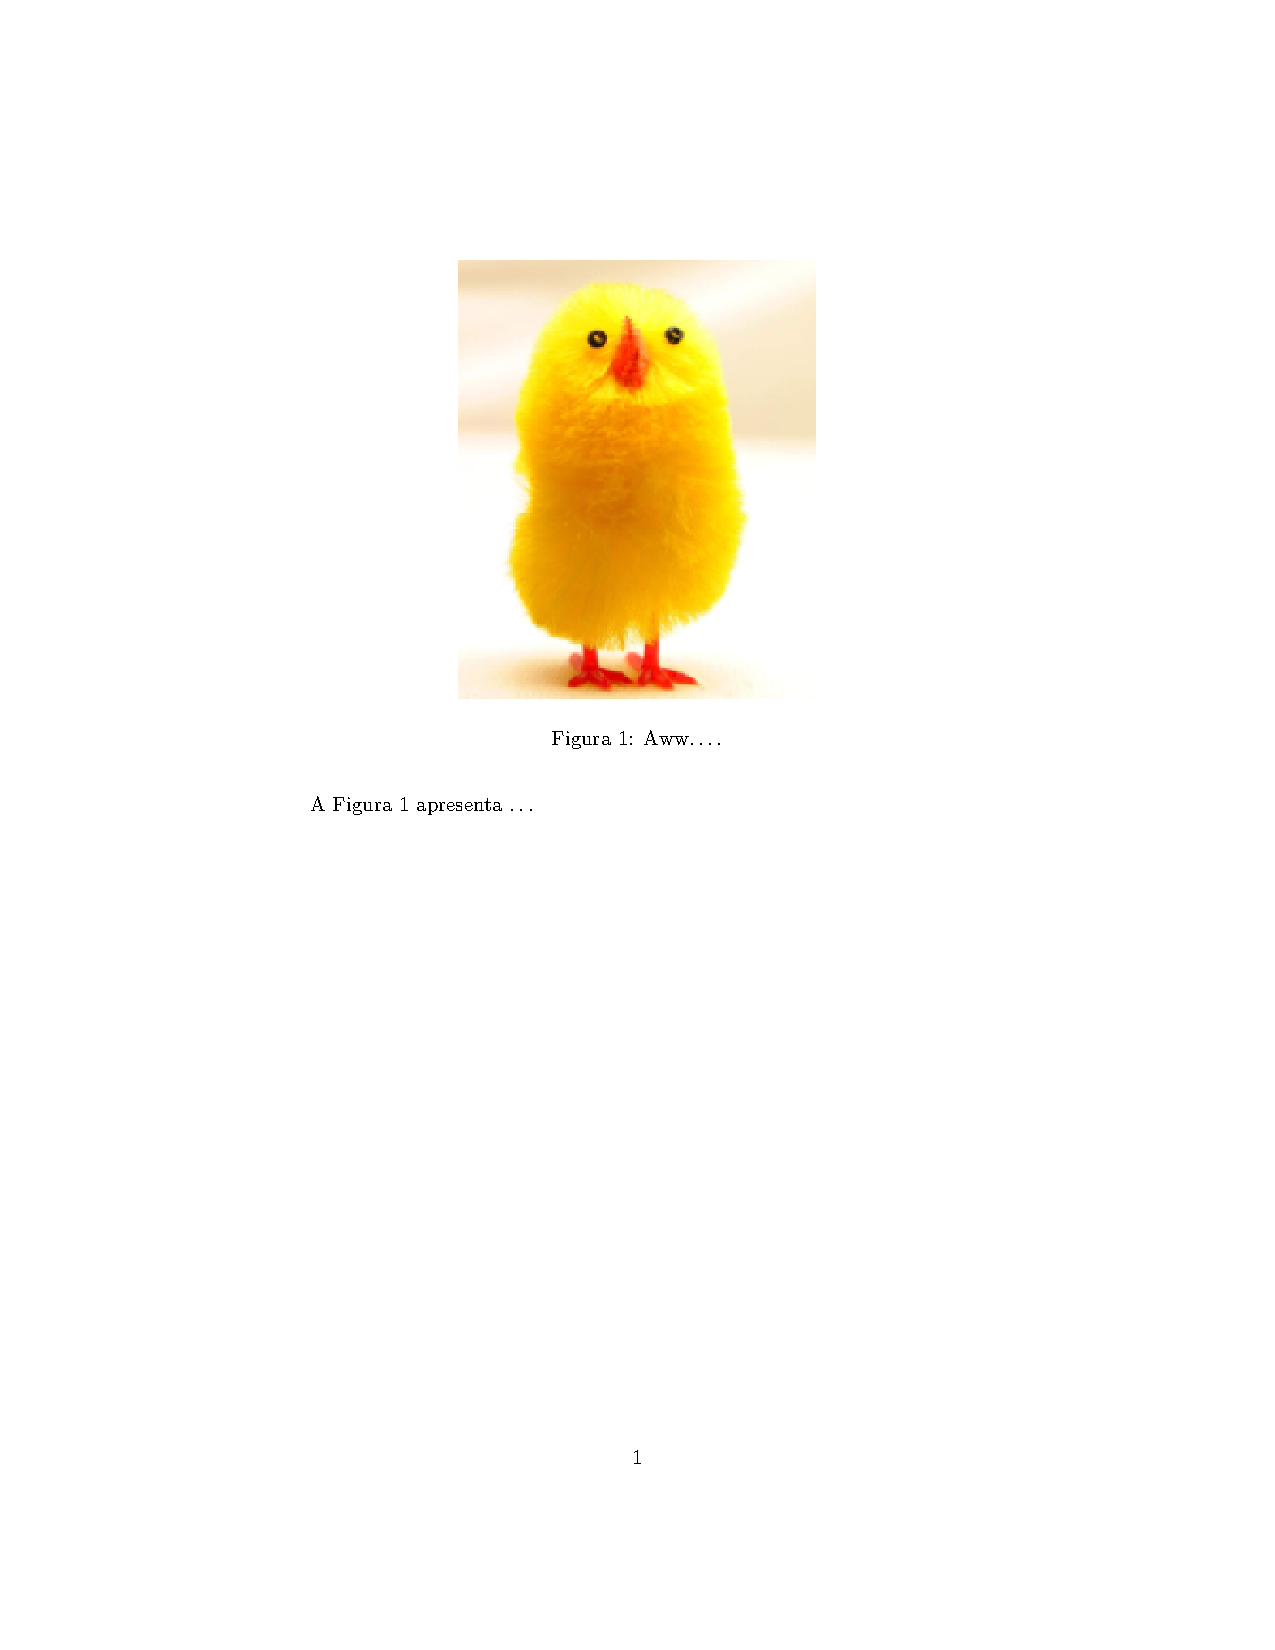
\includegraphics[width=\textwidth,clip,trim=2in 5in 3in 1in]{media-graphics.pdf}
	\end{minipage}
\end{frame}

%%%%%%%%%%%%%%%%%%%%%%%%%%%%%%%%%%%%%%%%%%%%%%%%%%%%%%%%%%%%%%%%%%%%%%%%%%%%%%%
%%%%%%%%%%%%%%%%%%%%%%%%%%%%%%%%%%%%%%%%%%%%%%%%%%%%%%%%%%%%%%%%%%%%%%%%%%%%%%%
%%%%%%%%%%%%%%%%%%%%%%%%%%%%%%%%%%%%%%%%%%%%%%%%%%%%%%%%%%%%%%%%%%%%%%%%%%%%%%%
\subsection{Tabelas}
\begin{frame}[fragile]{\insertsubsection}
	\begin{itemize}
		\item Leva um pouco de tempo para nos acostumarmos às tabelas em \LaTeX{} 
		\item Use o ambiente \bftt{tabular} definido no pacote \bftt{tabularx}.
		\item No argumento especificamos o alinhamento das colunas --- \textbf{l}eft, \textbf{r}ight, \textbf{r}ight.
		\begin{exampletwouptiny}
			\begin{tabular}{lrr}
				Item   & Qtd & R\$ \\
				Widget & 1   & 199,99  \\
				Gadget & 2   & 399,99  \\
				Cabo   & 3   & 19,99   \\
			\end{tabular}
		\end{exampletwouptiny}
		\item Use o e-comercial \keystrokebftt{\&} para separar as colunas e barra invertida dupla \keystrokebftt{\bs\bs} para começar uma nova linha (análogo ao ambiente \bftt{align*} que vimos na Parte 1 do curso).

	\end{itemize}
\end{frame}

\begin{frame}[fragile]{\insertsubsection}
	\begin{itemize}
		\item Também especificamos as linhas verticais com o símbolo \keystrokebftt{|} e as horizontais com o comando \cmdbs{hline}.
		
		\begin{exampletwouptiny}
			\begin{tabular}{|l|r|r|} 	\hline
				Item   & Qtd & R\$ 		\\ \hline
				Widget & 1   & 199,99  	\\
				Gadget & 2   & 399,99  	\\
				Cabo   & 3   & 19,99   	\\ \hline
			\end{tabular}
		\end{exampletwouptiny}
	\end{itemize}
\end{frame}

%%%%%%%%%%%%%%%%%%%%%%%%%%%%%%%%%%%%%%%%%%%%%%%%%%%%%%%%%%%%%%%%%%%%%%%%%%%%%%%
%%%%%%%%%%%%%%%%%%%%%%%%%%%%%%%%%%%%%%%%%%%%%%%%%%%%%%%%%%%%%%%%%%%%%%%%%%%%%%%
%%%%%%%%%%%%%%%%%%%%%%%%%%%%%%%%%%%%%%%%%%%%%%%%%%%%%%%%%%%%%%%%%%%%%%%%%%%%%%%
\addtocontents{toc}{\newpage}
\section{Bibliografia}

%%%%%%%%%%%%%%%%%%%%%%%%%%%%%%%%%%%%%%%%%%%%%%%%%%%%%%%%%%%%%%%%%%%%%%%%%%%%%%%
%%%%%%%%%%%%%%%%%%%%%%%%%%%%%%%%%%%%%%%%%%%%%%%%%%%%%%%%%%%%%%%%%%%%%%%%%%%%%%%
%%%%%%%%%%%%%%%%%%%%%%%%%%%%%%%%%%%%%%%%%%%%%%%%%%%%%%%%%%%%%%%%%%%%%%%%%%%%%%%
\begin{frame}{Conteúdo}
\begin{multicols}{2}
	\tableofcontents[currentsection]
\end{multicols}
\end{frame}

%%%%%%%%%%%%%%%%%%%%%%%%%%%%%%%%%%%%%%%%%%%%%%%%%%%%%%%%%%%%%%%%%%%%%%%%%%%%%%%
%%%%%%%%%%%%%%%%%%%%%%%%%%%%%%%%%%%%%%%%%%%%%%%%%%%%%%%%%%%%%%%%%%%%%%%%%%%%%%%
%%%%%%%%%%%%%%%%%%%%%%%%%%%%%%%%%%%%%%%%%%%%%%%%%%%%%%%%%%%%%%%%%%%%%%%%%%%%%%%
\subsection{bib\TeX}
\begin{frame}[fragile]{\insertsubsection{} 1}
	\begin{itemize}
		\item Coloque suas referências em um arquivo \bftt{.bib}, no formato `bibtex' :
		\inputminted[fontsize=\scriptsize,frame=single]{latex}{bib-example.bib}
		\item Diversos gerenciadores de referências podem exportar para o formato bibtex.
	\end{itemize}
\end{frame}

%%%%%%%%%%%%%%%%%%%%%%%%%%%%%%%%%%%%%%%%%%%%%%%%%%%%%%%%%%%%%%%%%%%%%%%%%%%%%%%
%%%%%%%%%%%%%%%%%%%%%%%%%%%%%%%%%%%%%%%%%%%%%%%%%%%%%%%%%%%%%%%%%%%%%%%%%%%%%%%
%%%%%%%%%%%%%%%%%%%%%%%%%%%%%%%%%%%%%%%%%%%%%%%%%%%%%%%%%%%%%%%%%%%%%%%%%%%%%%%
\begin{frame}[fragile]{\insertsubsection{} 2}
	\begin{itemize}
		\item Cada entrada no arquivo \bftt{.bib} recebe uma chave (\emph{key}) que você pode usar para referenciar no documento. Por exemplo, \bftt{Jacobson1999Towards} é a chave para este artigo:
		\begin{minted}[fontsize=\small,frame=single]{latex}
		@Article{Jacobson1999Towards,
		  author = {Van Jacobson},
		  ...
		}
		\end{minted}
		\item É uma boa ideia usar chaves baseadas no nome, ano e título da obra.
		\item \LaTeX{} pode formatar suas citações no texto e gerar a lista de referências automaticamente; Ele reconhece a maioria dos estilos padrão, e você ainda pode definir o seu próprio.
	\end{itemize}
\end{frame}

%%%%%%%%%%%%%%%%%%%%%%%%%%%%%%%%%%%%%%%%%%%%%%%%%%%%%%%%%%%%%%%%%%%%%%%%%%%%%%%
%%%%%%%%%%%%%%%%%%%%%%%%%%%%%%%%%%%%%%%%%%%%%%%%%%%%%%%%%%%%%%%%%%%%%%%%%%%%%%%
%%%%%%%%%%%%%%%%%%%%%%%%%%%%%%%%%%%%%%%%%%%%%%%%%%%%%%%%%%%%%%%%%%%%%%%%%%%%%%%
\begin{frame}[fragile]{\insertsubsection{} 3}
	\begin{itemize}
		\item Use o pacote \bftt{natbib} (recomendado).
		\item Use \cmdbs{citet} e \cmdbs{citep} para inserir citações por chaves.
		\item Referencie \cmdbs{bibliography} no final do documento, e especifique um estilo (\cmdbs{bibliographystyle}).
	\end{itemize}
	\begin{minipage}{0.55\linewidth}
	\inputminted[fontsize=\tiny,frame=single,resetmargins]{latex}%
	  {bib-example.tex}
	\end{minipage}
	\begin{minipage}{0.35\linewidth}
		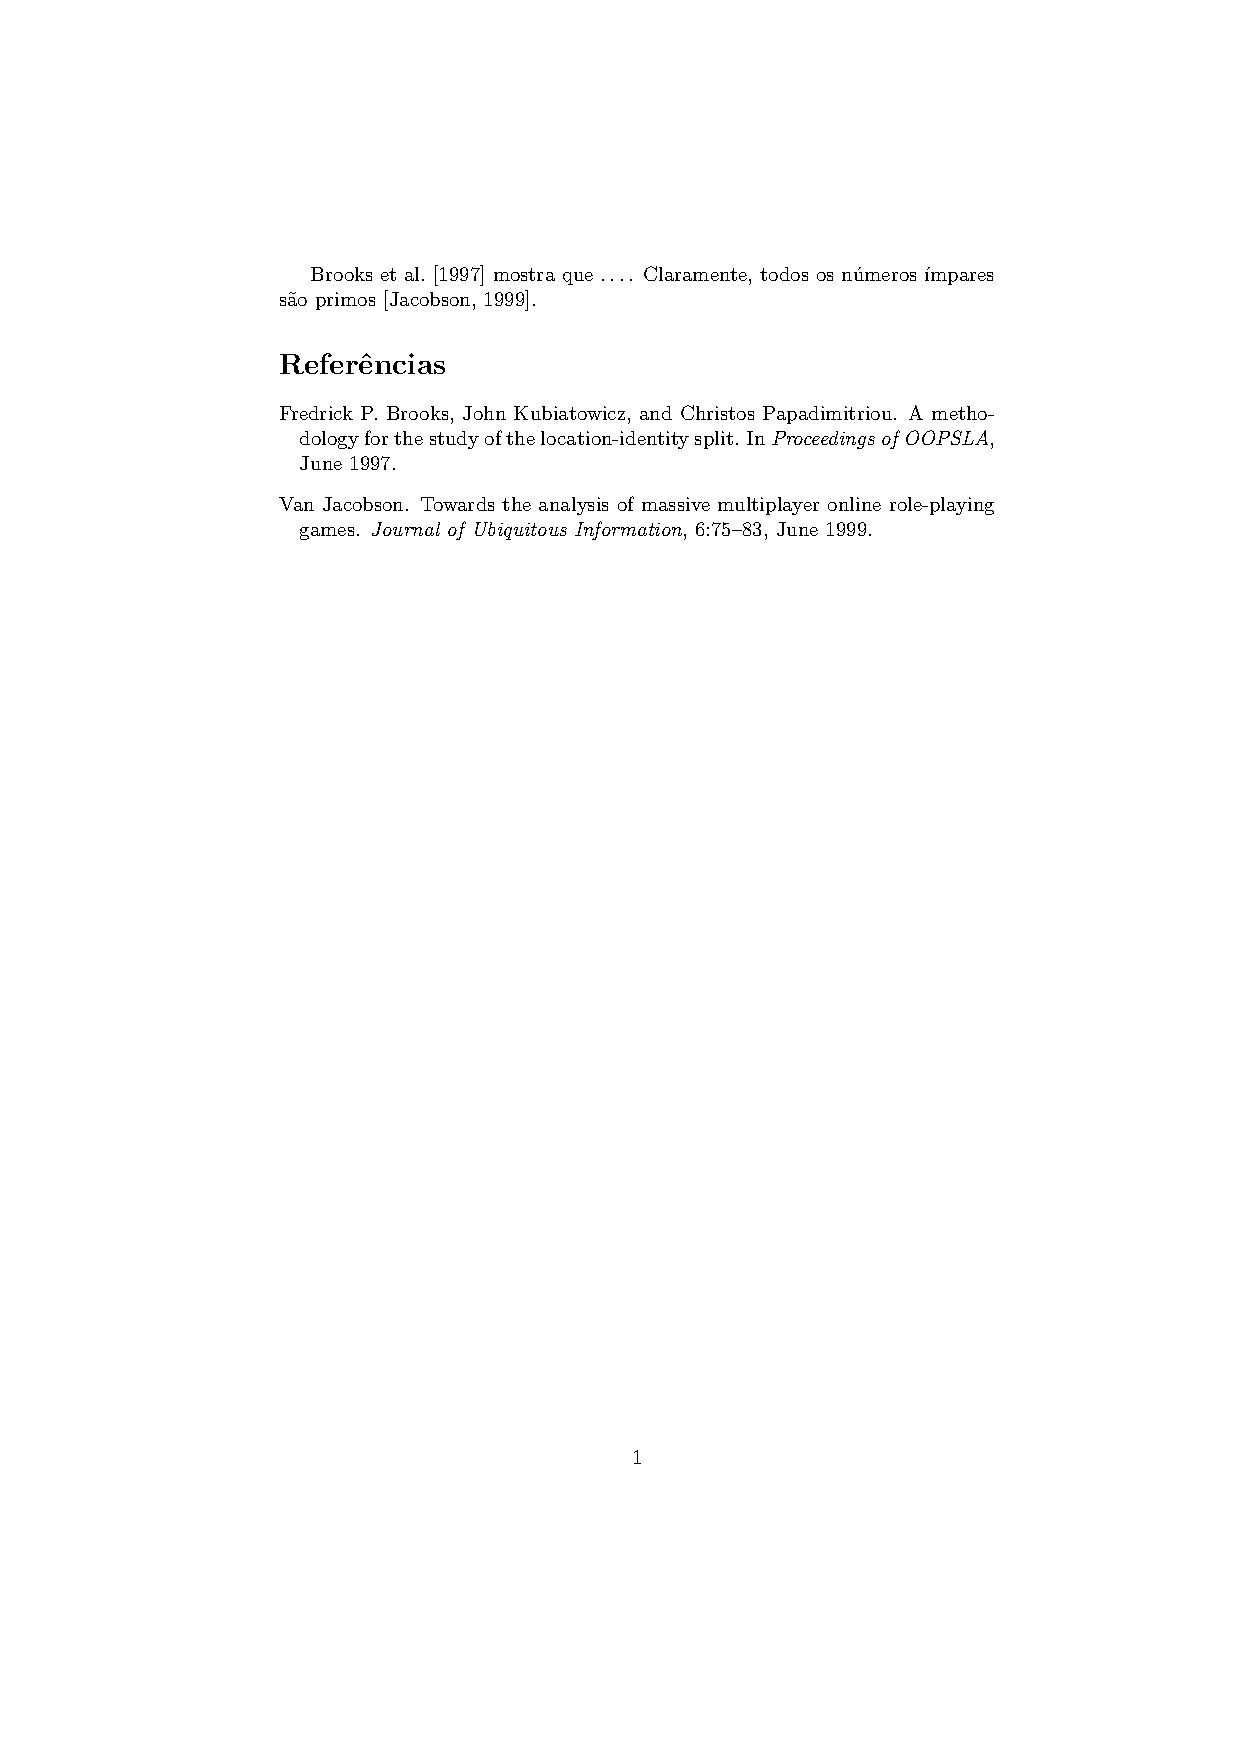
\includegraphics[width=\textwidth,clip,trim=1.8in 5in 1.8in 1in]{bib-example.pdf}
	\end{minipage}
\end{frame}

%%%%%%%%%%%%%%%%%%%%%%%%%%%%%%%%%%%%%%%%%%%%%%%%%%%%%%%%%%%%%%%%%%%%%%%%%%%%%%%
%%%%%%%%%%%%%%%%%%%%%%%%%%%%%%%%%%%%%%%%%%%%%%%%%%%%%%%%%%%%%%%%%%%%%%%%%%%%%%%
%%%%%%%%%%%%%%%%%%%%%%%%%%%%%%%%%%%%%%%%%%%%%%%%%%%%%%%%%%%%%%%%%%%%%%%%%%%%%%%
\subsection{Exercise}
\begin{frame}[fragile]{Exercício: Colocando tudo junto}

Adicione uma imagem e a bibliografia ao artigo do exercício anterior.


\begin{enumerate}
\item Baixe esses arquivos de exemplo para o seu computador.

\begin{center}
\fbox{\href{\fileuri/big_chick.png?dl=1}{Clique aqui para baixar a imagem exemplo}}

\fbox{\href{\fileuri/bib-exercise.bib?dl=1}{Clique aqui para baixar o arquivo bib exemplo}}
\end{center}

\item Carregue-os no writeLaTeX (use o menu ``files'').

\item Para encontrar as chaves no arquivo \bftt{.bib}, você terá que abri-lo em um editor de texto no seu computador --- você não pode vê-lo online via writeLaTeX, ainda.

\end{enumerate}
\end{frame}

%%%%%%%%%%%%%%%%%%%%%%%%%%%%%%%%%%%%%%%%%%%%%%%%%%%%%%%%%%%%%%%%%%%%%%%%%%%%%%%
%%%%%%%%%%%%%%%%%%%%%%%%%%%%%%%%%%%%%%%%%%%%%%%%%%%%%%%%%%%%%%%%%%%%%%%%%%%%%%%
%%%%%%%%%%%%%%%%%%%%%%%%%%%%%%%%%%%%%%%%%%%%%%%%%%%%%%%%%%%%%%%%%%%%%%%%%%%%%%%
\section{O que há na sequência?}

%%%%%%%%%%%%%%%%%%%%%%%%%%%%%%%%%%%%%%%%%%%%%%%%%%%%%%%%%%%%%%%%%%%%%%%%%%%%%%%
%%%%%%%%%%%%%%%%%%%%%%%%%%%%%%%%%%%%%%%%%%%%%%%%%%%%%%%%%%%%%%%%%%%%%%%%%%%%%%%
%%%%%%%%%%%%%%%%%%%%%%%%%%%%%%%%%%%%%%%%%%%%%%%%%%%%%%%%%%%%%%%%%%%%%%%%%%%%%%%
\begin{frame}{Conteúdo}
\begin{multicols}{2}
	\tableofcontents[currentsection]
\end{multicols}
\end{frame}

%%%%%%%%%%%%%%%%%%%%%%%%%%%%%%%%%%%%%%%%%%%%%%%%%%%%%%%%%%%%%%%%%%%%%%%%%%%%%%%
%%%%%%%%%%%%%%%%%%%%%%%%%%%%%%%%%%%%%%%%%%%%%%%%%%%%%%%%%%%%%%%%%%%%%%%%%%%%%%%
%%%%%%%%%%%%%%%%%%%%%%%%%%%%%%%%%%%%%%%%%%%%%%%%%%%%%%%%%%%%%%%%%%%%%%%%%%%%%%%
\subsection{Mais coisas interessantes}
\begin{frame}[fragile]{\insertsubsection}
	\begin{itemize}
		\item Adicione o comando \cmdbs{tableofcontents} para gerar o sumário a partir dos comandos \cmdbs{section}.
		
		\item Altere o comando \cmdbs{documentclass} para
		\mint{latex}!\documentclass{scrartcl}!
		or
		\mint{latex}!\documentclass[12pt]{IEEEtran}!
		
		\item Defina seus próprios comandos para equações complexas:
		\begin{exampletwouptiny}
		\newcommand{\rperf}{%
		  \rho_{\text{perf}}}
		$$
		\rperf = {\bf c}'{\bf X} + \varepsilon
		$$
		\end{exampletwouptiny}
	\end{itemize}
\end{frame}

%%%%%%%%%%%%%%%%%%%%%%%%%%%%%%%%%%%%%%%%%%%%%%%%%%%%%%%%%%%%%%%%%%%%%%%%%%%%%%%
%%%%%%%%%%%%%%%%%%%%%%%%%%%%%%%%%%%%%%%%%%%%%%%%%%%%%%%%%%%%%%%%%%%%%%%%%%%%%%%
%%%%%%%%%%%%%%%%%%%%%%%%%%%%%%%%%%%%%%%%%%%%%%%%%%%%%%%%%%%%%%%%%%%%%%%%%%%%%%%
\subsection{Mais pacotes interessantes}
\begin{frame}{\insertsubsection}
	\begin{itemize}
		\item \bftt{beamer}: para apresentações (como essa aqui!)
		\item \bftt{todonotes}: comentários e gerenciamento de tarefas (TODO management)
		\item \bftt{tikz}: para construção de gráficos (figuras) maravilhosos
		\item \bftt{pgfplots}: criação de gráficos (charts) diretamente em \LaTeX
		\item \bftt{spreadtab}: criação de planilhas eletrônicas em \LaTeX
		\item \bftt{gchords}, \bftt{guitar}: acordes de violão e guitarra
		\item \bftt{cwpuzzle}: palavras cruzadas
	\end{itemize}
	Veja \url{https://www.writelatex.com/examples} e \url{http://texample.net} para
	exemplos de desses pacores.
\end{frame}

%%%%%%%%%%%%%%%%%%%%%%%%%%%%%%%%%%%%%%%%%%%%%%%%%%%%%%%%%%%%%%%%%%%%%%%%%%%%%%%
%%%%%%%%%%%%%%%%%%%%%%%%%%%%%%%%%%%%%%%%%%%%%%%%%%%%%%%%%%%%%%%%%%%%%%%%%%%%%%%
%%%%%%%%%%%%%%%%%%%%%%%%%%%%%%%%%%%%%%%%%%%%%%%%%%%%%%%%%%%%%%%%%%%%%%%%%%%%%%%
\subsection{Instalando \LaTeX{}}
\begin{frame}{\insertsubsection}
	\begin{itemize}
		\item Para rodar \LaTeX{} no seu computador, você precisa de uma distribuição \LaTeX{}, que inclui o programa \bftt{latex} e (tipicamente) centenas de pacotes.
			\begin{itemize}
				\item Windows: \href{http://miktex.org/}{Mik\TeX}
				\item Linux: \href{http://tug.org/texlive/}{\TeX Live}
				\item Mac: \href{http://tug.org/mactex/}{Mac\TeX}
			\end{itemize} 
		\item Você também vai querer um editor com suporte ao \LaTeX{}. Veja uma lista com (muitas) opções em {\scriptsize \url{http://en.wikipedia.org/wiki/Comparison_of_TeX_editors}}.
		\item Você terá que aprender mais sobre como \bftt{latex} e suas ferramentas relacionadas trabalham --- veja os recursos no próximo slide.
	\end{itemize}
\end{frame}

%%%%%%%%%%%%%%%%%%%%%%%%%%%%%%%%%%%%%%%%%%%%%%%%%%%%%%%%%%%%%%%%%%%%%%%%%%%%%%%
%%%%%%%%%%%%%%%%%%%%%%%%%%%%%%%%%%%%%%%%%%%%%%%%%%%%%%%%%%%%%%%%%%%%%%%%%%%%%%%
%%%%%%%%%%%%%%%%%%%%%%%%%%%%%%%%%%%%%%%%%%%%%%%%%%%%%%%%%%%%%%%%%%%%%%%%%%%%%%%
\subsection{Recursos Online}
\begin{frame}{\insertsubsection}
	\begin{itemize}
		\item \href{http://en.wikibooks.org/wiki/LaTeX}{The \LaTeX{} Wikibook} ---
		tutoriais excelentes e material de referência.
		\item \href{http://tex.stackexchange.com/}{\TeX{} Stack Exchange} --- faça perguntas e receba respostas excelentes e incrivelmente rápidas
		\item \href{http://www.latex-community.org/}{\LaTeX{} Community} --- Um grande fórum 
		online
		\item \href{http://ctan.org/}{Comprehensive \TeX{} Archive Network (CTAN)} ---
		mais de 4 mil pacotes e respectiva documentação
		\item Google usualmente vai te mandar para um itens acima.
	\end{itemize}
\end{frame}

%%%%%%%%%%%%%%%%%%%%%%%%%%%%%%%%%%%%%%%%%%%%%%%%%%%%%%%%%%%%%%%%%%%%%%%%%%%%%%%
%%%%%%%%%%%%%%%%%%%%%%%%%%%%%%%%%%%%%%%%%%%%%%%%%%%%%%%%%%%%%%%%%%%%%%%%%%%%%%%
%%%%%%%%%%%%%%%%%%%%%%%%%%%%%%%%%%%%%%%%%%%%%%%%%%%%%%%%%%%%%%%%%%%%%%%%%%%%%%%
\begin{frame}
\begin{center}
	Obrigado, e feliz \TeX{}ing!
\end{center}
\end{frame}

\end{document}

% -- latex understands words, sentences and paragraphs

Words are separated by one or more spaces.  Paragraphs are separated by
one or more blank lines.  The output is not affected by adding extra
spaces or extra blank lines to the input file.

Double quotes are typed like this: ``quoted text''.
Single quotes are typed like this: `single-quoted text'.

Emphasized text is typed like this: \emph{this is emphasized}.
Bold       text is typed like this: \textbf{this is bold}.

-- Adding structure to your document

\section{Hello}

\subsection{World}

\subsection{Foo}

\subsubsection*{Stuff} % star form

\subsubsection*{Results}

-- Labels and cross-references

\label{sec:intro}
\label{sec:method}
\ref{sec:method}

--> maybe introduce the prettyref package here.

-- Mathematics

Inline mathematics: $x + y < 7$.

'Displayed' mathematics:
\begin{equation}
\end{equation}

\begin{equation*}
\end{equation*}

\begin{align}
\end{align}

-- Figures

- Need the graphicx package.

- here we can start introducing options

\includegraphics[width=\textwidth]{}

- where do you find out about these options? --> link to the Wikibook

-- Floating Figures

\begin{figure}
\includegraphics{...}
\caption{\label{}Here is a caption.}
\end{figure}

-- Tables

- not the nicest part of LaTeX

\usepackage{tabularx}

\begin{tabular}{llr}
Item & Quantity & Price (\$) & Amount
Widget & 1 & 
\end{tabular}

Bonus points: check out the fp package and the spreadtab package.

-- Document Classes

a .cls file

article

some journal templates come with one

-- Bibliographies



-- For Typesetting Geeks

- dashes: -, --, ---

- ellipsis.

- controlling spaces: ~, \ , \,, \@

- spacing after periods (et al., etc.)

- Nested quotation marks: ``\,`
\vskip 2ex
\item Use the \emph{star form} to display an equation without a number.
\begin{exampletwouptiny}
\begin{equation*}
F(x) = \int_{a}^{x}{f(t) dt}
\end{equation*}
\end{exampletwouptiny}

\begin{itemize}
\item \bftt{equation} and \bftt{equation*} are called \emph{environments}.
\begin{itemize}
  \item The \cmdbs{begin} and \cmdbs{end} commands define the environment.
  \item The \cmd{\$} also starts and ends an environment.
  \item Some commands are defined only within certain environments.
  \item Some commands behave differently in different environments.
\end{itemize}
\end{itemize}
\end{block}
\begin{center}
\fbox{\href{http://ctan.org/}{The Comprehensive \TeX Archive Network (CTAN)}}
\end{center}

%%%%%%%%%%%%%%%%%%%%%%%%%%%%%%%%%%%%%%%%%%%%%%%%%%%%%%%%%%%%%%%%%%%%%%%%%%%%%%%
%%%%%%%%%%%%%%%%%%%%%%%%%%%%%%%%%%%%%%%%%%%%%%%%%%%%%%%%%%%%%%%%%%%%%%%%%%%%%%%
%%%%%%%%%%%%%%%%%%%%%%%%%%%%%%%%%%%%%%%%%%%%%%%%%%%%%%%%%%%%%%%%%%%%%%%%%%%%%%%
\subsection{Typography tweaks}
\begin{frame}{\insertsubsection}
\begin{tabular}{lll}
& character name & used mainly for \ldots \\\hline
\bftt{\bs} & backslash                 & commands, tables \\
\bftt{\{}  & open brace                & commands \\
\bftt{\}}  & close brace               & commands \\
\bftt{\%}  & percent sign              & comments \\
\bftt{\#}  & hash (pound / sharp) sign & custom commands \\
\bftt{\$}  & dollar sign               & equations \\
\bftt{\_}  & underscore                & equations (subscripts) \\
\bftt{\^}  & caret                     & equations (superscripts) \\
\bftt{\&}  & ampersand                 & tables \\
\bftt{\~}  & tilde                     & spacing \\
\end{tabular}
\end{frame}

%\item We've used several environments:
%\vskip 1ex
%{\scriptsize
%\begin{tabular}{ll}
%\cmdbs{begin}\bftt{\{document\}}\ldots\cmdbs{end}\bftt{\{document\}} &
%  document environment \\
%\cmdbs{begin}\bftt{\{itemize\}}\ldots\cmdbs{end}\bftt{\{itemize\}} &
%  itemized list environment \\
%\bftt{\$\ldots\$}     & \emph{in-text} math environment \\
%\bftt{\$\$\ldots\$\$} & \emph{displayed} math environment \\
%\cmdbs{begin}\bftt{\{equation\}}\ldots\cmdbs{end}\bftt{\{equation\}} &
%  displayed math environment w/ number
%\end{tabular}
%}

